\documentclass[10pt]{dokument-ppi}

\begin{document}


\Cwiczenie{Ćwiczenie 2}
\Meta
\Tytul{Macierz odpowiedzialności}
\Data{2012-11-07}
\Autorzy{TC}
\MakeDokumentMeta


\section{Macierz odpowiedzialności}

Znajduje się na stronie \pageref{fig:macierz}.

\begin{figure}[p]
    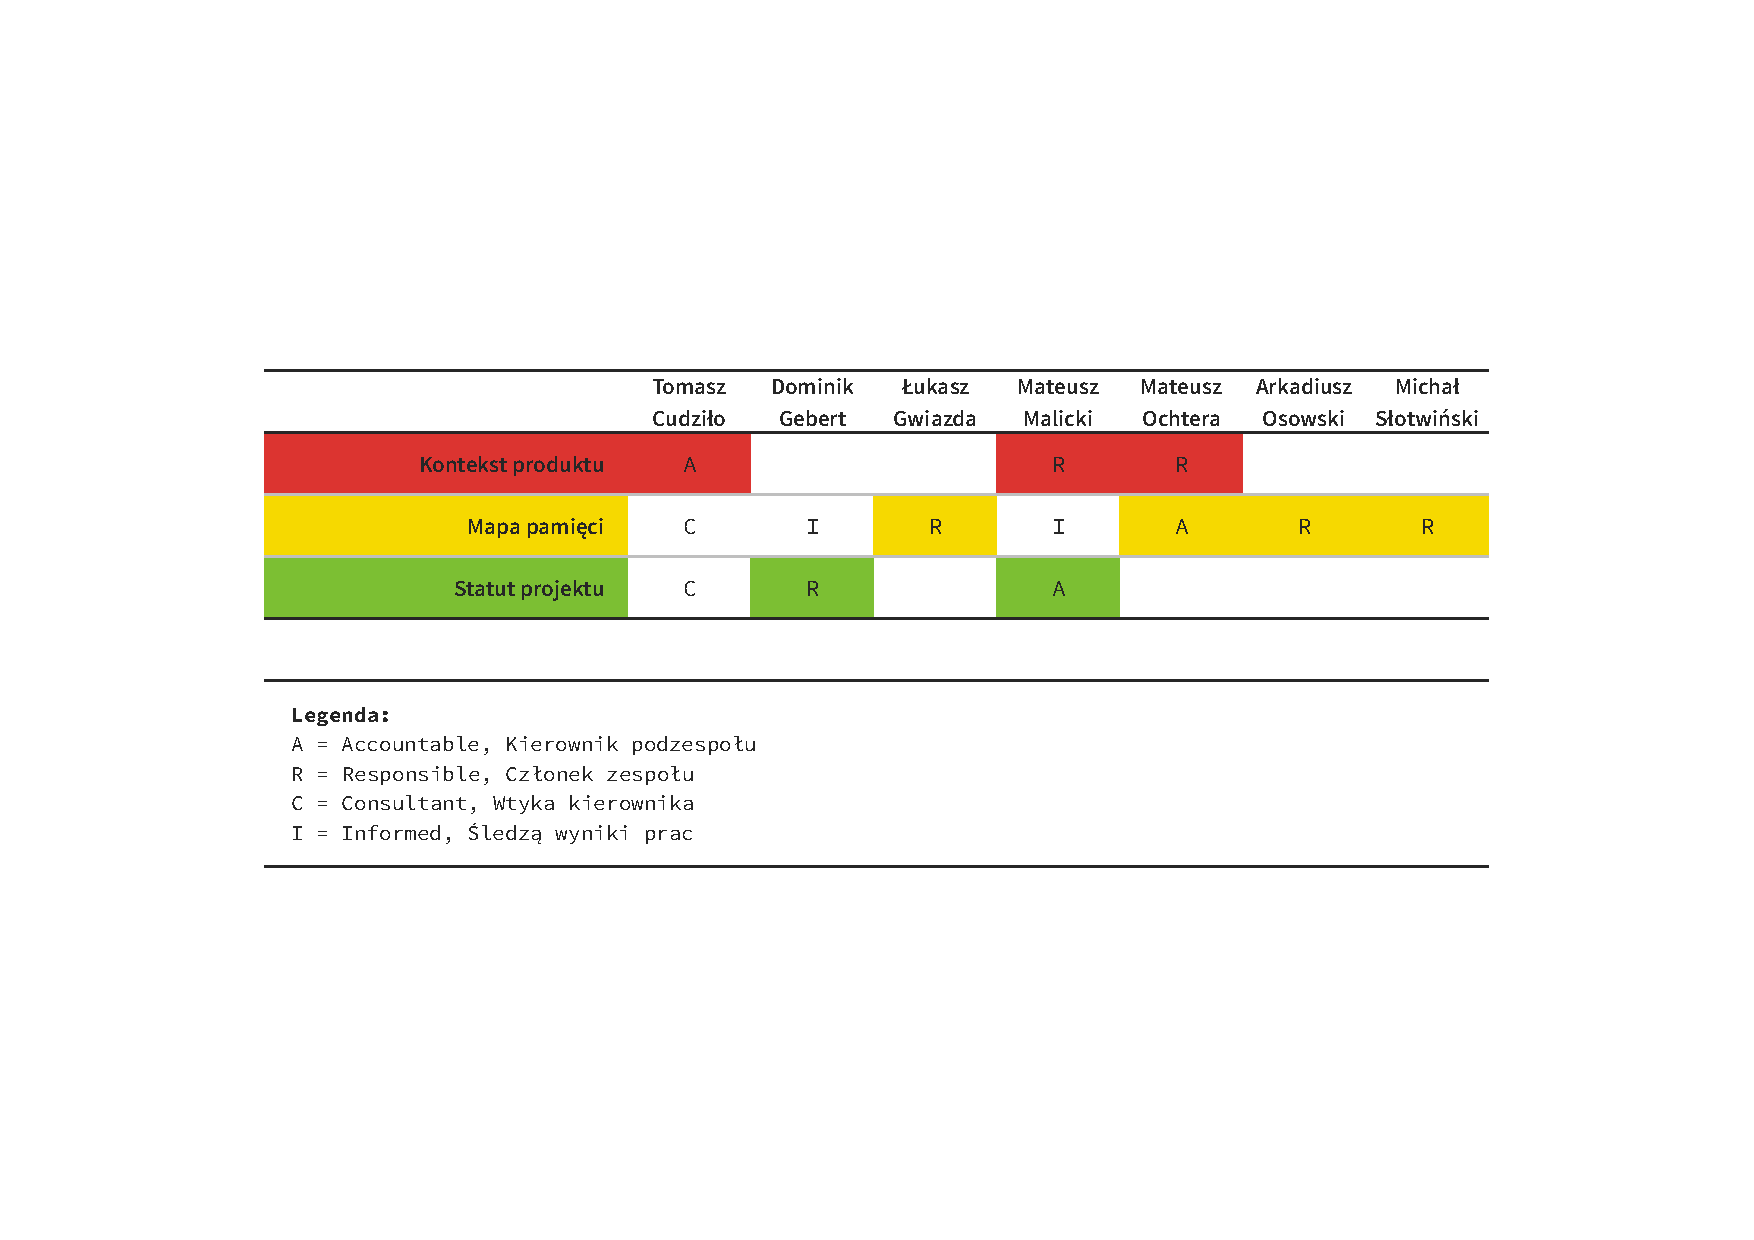
\includegraphics[page=1, angle=270, scale=0.75, clip=true]{./figury/macierz-odpowiedzialnosci}
    \caption{Macierz odpowiedzialności za dokumenty tworzone w ramach ćwiczenia 2.}
    \label{fig:macierz}
\end{figure}


\section{Historia dokumentu}
\begin{versions}
    \version*{1.0}{2012-11-07}{TC}%
        Dodano pełną macierz odpowiedzialności.
\end{versions}


\end{document}
